\documentclass[12pt,a4paper]{article}
\usepackage[german]{babel}
\usepackage[utf8]{inputenc}
\usepackage{amsmath, amsthm, amssymb}
\usepackage{enumerate}
\usepackage{graphicx}
\usepackage{pdflscape}
\usepackage{setspace}
\onehalfspacing
\usepackage{wrapfig}
\usepackage{hyperref}
\usepackage{multirow}
\usepackage[round]{natbib}
\bibliographystyle{apalike}

\newtheorem{definition}{Definition}[section]
\newtheorem{interview}{Interview}[section]
\newtheorem{satz}{Satz}[section]
\newtheorem{beispiel}{Beispiel}[section]
\newtheorem{bemerkung}{Bemerkung}[section]
\newtheorem{literaturverzeichnis}{Literaturverzeichnis}[section]

\usepackage[top=25mm, bottom=20mm, vmargin=25mm, includehead]{geometry} % Document Margins
\setlength{\topmargin}{0cm}
\setlength{\parindent}{5mm}
\setlength{\parskip}{2mm}
\setlength{\evensidemargin}{0mm}
\setlength{\oddsidemargin}{0cm}
%\pagestyle{headings}


\begin{document}
\thispagestyle{empty}
\vspace*{-3cm}
\begin{center}
\includegraphics[width=\textwidth]{htw.pdf}
\vspace{0.5cm}
\hrule
\vspace{5.5cm}
{\Large \textsc{Belegabeit\\
Internettechnologien II}}\\
{\large WS 2020/21}\\
\vspace{1cm}
{\Large \bf
RTSP-Streaming}\\
\vspace*{1cm}
{\large Dozent:  Prof. Dr.-Ing. Jörg Vogt}
\end{center}
\vspace*{5cm}
{\large

\hspace*{7cm}
\parbox{8.2cm}
{
\begin{tabular}{ll}
Vorgelegt von & Felix Müller\\
& s79138\\
Abgabetermin: & 17.01.2021

\end{tabular}}}

\newpage
\pagenumbering{arabic}
\tableofcontents

\newpage
\section{Parameterwahl}\label{intro}

\subsection{Rechnung}

\begin{itemize}
	\item Es wird angenommen, dass die Frameverluste binomialverteilt und voneinander unabhängig sind.
	\item Als Kanalfehlerwahrscheinlichkeit wird $P_e = 0,1$ verwendet.
\end{itemize}

Nimmt man an, dass ein Video mit einer Bildwiederholrate ab $24 \textrm{ Hz}$ von den meisten Menschen als ruckelfrei wahrgenommen wird, so darf höchstens ein Frame pro Sekunde verloren gehen. Gesucht ist also die Paketfehlerwahrscheinlichkeit $P_r$ für $n = 25$ und den Erwartungswert $\mathbb{E}(n) = 24$.
$$\mathbb{E} = n \cdot P_r \rightarrow P_r = 0,96$$

Mithilfe der Formel für den Restfehler in 2. ergibt sich damit eine FEC-Gruppengröße von $k = 2$\\

Nimmt man higegen an, dass ein Video mit einer Bildwiederholrate von $18 \textrm{ Hz}$ zwar als ruckelig aber dennoch als bewegtes Bild wahrgenommen wird, ergibt sich, dass eine FEC-Gruppengröße von 48 genügt. Die Restfehlerwahrscheinlichkeit nach der FEC-Korrektur beträgt dann $P_r \approx 0,1$, der Erwartungswert für die mögliche Bildwiederholrate also $\mathbb{E} \approx 0,9 \cdot n = 22,5$

\subsection{Beobachtung}

Die Wiedergabe eines mit diesen Parametern gestreamten Videos bestätigt die Berechnung, auch subjektiv scheint die Videoqualität mit $k=48$ ausreichend zu sein. 

\section{Bestimmung der theoretisch zu erwartenden Verlustraten}

Gesucht ist das Ereignis $A \dots$ Paketverlust nach FEC-Fehlerkorrektur, seine Wahrscheinlichkeit lässt sich durch sein Gegenereignis $\bar{A} \dots$ kein Verlust eines Pakets nach FEC-Fehlerkorrektur bestimmen. $\bar{A}$ besteht aus den Ereignisen:

\begin{itemize}
	\item $B \dots$ das Paket ist fehlerfrei übertragen worden $$P(B) = 1 - P_e$$
	\item $C \dots$ das Paket ist nicht übertragen worden, kann aber durch den FEC-Mechanismus wiederhergestellt werden, das bedeutet dass alle anderen $k$ Pakete der FEC-Gruppe der Größe $k$ fehlerfrei übertragen worden $$P(C) = P_e \cdot (1 - P_e)^k$$
\end{itemize}

Die Wahrscheinlichkeit für $A$ beträgt also: $$P(A) = 1 - (1 - P_e) + (P_e \cdot (1 - P_e)^k) = - P_e \cdot \biggl( \bigl[ - (P_e - 1) \bigr]^k - 1 \biggr)$$

Die Restfehlerhäufigkeit kann durch severseitige Simulation von Paketfehlern auch gemessen werden. 

\begin{tabular}{c||c|c|c|c|c}
	Paketfehlerwahrscheinlichkeit & $10\%$ & $20\%$ & $30\%$ & $40\%$ & $50\%$ \\
	\hline
	Gruppengröße & \multicolumn{5}{|c}{Restfehlerhäufigkeit} \\
	\hline \hline
	$2$ &  $0,0217$ & $0,0797$ & $0,1650$ & $0,2553$ & $0,3695$\\
	$48$ & $0,1046$ & $0,2048$ & $0,3062$ & $0,3962$ & $0,4922$
\end{tabular}

\begin{landscape}

\newpage
\begin{figure}[h]
	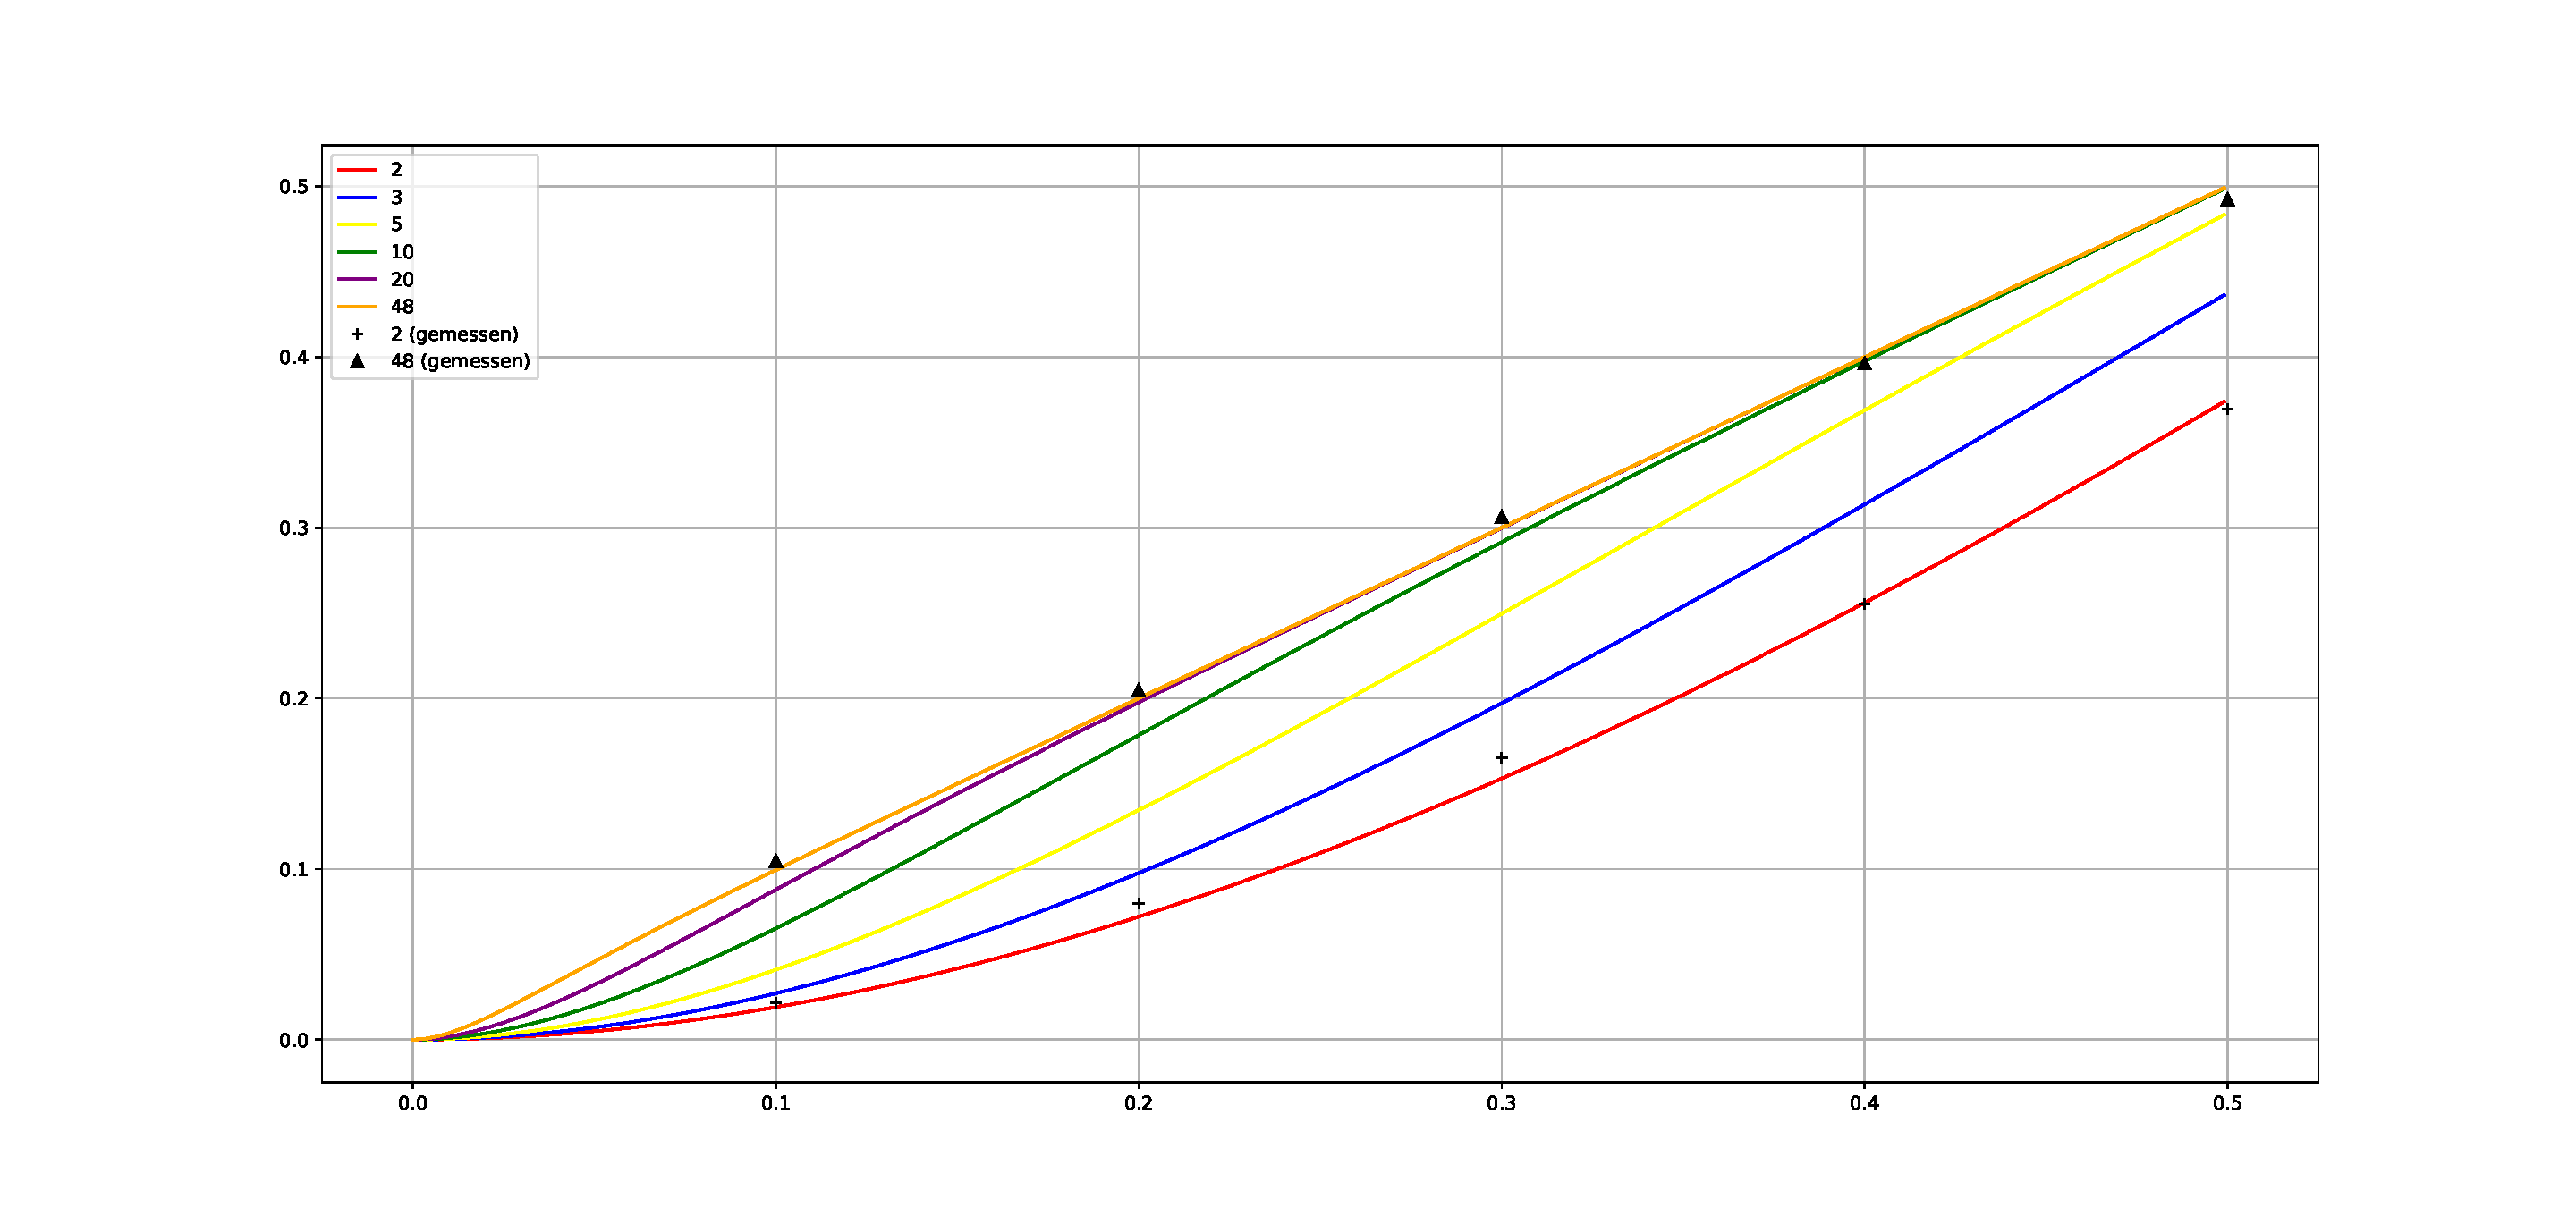
\includegraphics[width=21cm]{Plot_Restfehler.pdf}
	\caption{theoretische Restfehlerwahrscheinlichkeit und gemessene Restfehlerhäufigkeit in Abhängigkeit der Gruppengröße}
\end{figure}

\end{landscape}

\section{Kompatibilität}

\subsection{VLC als Client}

Wird versucht VLC als Client zu benutzen, funktioniert das bis zum RTSP-\textsc{describe}. VLC schließt die Verbindung nach Erhalt der \textsc{describe}-Response vom Server und gibt folgende Fehlermeldung aus: \glqq unable to connect to RTSP server\grqq{}

\subsection{VLC als Server}

\begin{itemize}
\item Version 3.x\\
Als Response auf den \textsc{setup}-Request folgt: \glqq RTSP/1.0 500 Server error\grqq{}\\
Die Ursache lässt sich nicht bestimmen.
\end{itemize}

\section{Vorschläge zur Verbesserung}

\begin{itemize}
\item Die Größe der RTP-Pakete sollte auf die MTU begrenzt werden, um Fragmentierung im IP-Layer des Netzwerkstacks zu verhindern, ein verlorenes IP-Paket bedeutet sonst den Verlust aller zu einem RTP-Paket gehörenden IP-Pakete.
\item Die Fehlersimulation sollte sich auf IP-Pakete beziehen und nicht auf gesamte RTP-Pakete. (siehe oben)
\item Die Implementierung einer Fehlerverdeckung würde die QoS weiter verbessern.
\end{itemize}

\end{document}

